% !TEX program = xelatex
%%%%%%%%%%%%%%%%%%%%%%%%

\documentclass[11pt,aspectratio=169]{beamer} % 11pt is default
\usetheme{metropolis} % [progressbar=frametitle]
\setbeamercolor{background canvas}{bg=white}
\setbeamertemplate{caption}{\insertcaption} 
\setbeamersize{text margin left=2em,text margin right=2em}
\setbeamertemplate{frame footer}{\vspace{-5pt}}

\usepackage[round]{natbib}
\usepackage{amsmath}
\usepackage{mathtools}
\usepackage[group-minimum-digits=4,group-separator={,}]{siunitx}
\usepackage{graphicx}
\usepackage{wrapfig}
\usepackage{multimedia}

\usepackage{tikz}
\usetikzlibrary{backgrounds}
\usetikzlibrary{arrows,shapes}
\usetikzlibrary{tikzmark}
\usetikzlibrary{calc}
\usepackage[dvipsnames]{xcolor}

\usepackage[skins,theorems]{tcolorbox}
\usepackage{pdfpages}
\usepackage{colortbl}
\usepackage{changepage}
\usepackage{booktabs}
\usepackage{makecell}
\usepackage{setspace}
\usepackage{algorithm}
\usepackage[noend]{algpseudocode}
\usepackage{subcaption}
\usepackage[framemethod=TikZ]{mdframed}
\usepackage{xspace}

\usepackage{annotate-equations}

% Shortcut for beamer frames
\newcommand{\bframe}[2][c]{\begin{frame}[#1]{#2}}
\newcommand{\eframe}{\end{frame}} % \eframe causes problems for some reason

% Shortcut for bold text
\newcommand{\fat}[1]{\textbf{#1}}

% Boxing items on slide
\newcommand{\Cboxed}[2]{\colorlet{currentcolor}{.}{\color{#1}\fbox{\color{currentcolor}#2}}} %create coloured box around equation

% checkmark and xmark
\usepackage{pifont}
\newcommand{\cmark}{\ding{51}}%
\newcommand{\xmark}{\ding{55}}%

% Highlighting text in orange
\newcommand{\e}[1]{\alert{#1}}

% Underline
\newcommand{\uline}[1]{\underline{#1}}

% Include figure
\newcommand{\imgw}[2]{\includegraphics[width=#2\textwidth]{#1}} % \imgw{file}{height-scale}
\newcommand{\imgh}[2]{\includegraphics[height=#2\textheight]{#1}} % \imgh{file}{width-scale}

% Shortcut for latex commands
\newcommand{\blist}{\vspace{-3pt}\begin{list}{\raisebox{1pt}{\small$\bullet$}}{\leftmargin=13pt\itemsep=4pt}}
\newcommand{\blisttab}{\vspace{5pt}\blist}
\newcommand{\elisttab}{\end{list}}
\newcommand{\listtab}{\\[3pt] $\Rightarrow$ }
\newcommand{\elist}{\end{list}\vspace{5pt}}
\newcommand{\bblock}[1]{\metroset{block=fill}\begin{block}{#1}}
\newcommand{\eblock}{\end{block}}
\newcommand{\bmath}[1][0]{\begin{equation*}\hspace{#1em}}
\newcommand{\emath}{\end{equation*}}
\newcommand{\bcol}{\begin{columns}}
\newcommand{\col}[1]{\column{#1\textwidth}}
\newcommand{\tcol}[1]{\column[T]{#1\textwidth}}
\newcommand{\ecol}{\end{columns}}
\newcommand{\place}[4]{\begin{textblock}{#3}(#1,#2) #4 \end{textblock}} % \place{x}{y}{width}{text}
\newcommand{\placeframed}[4]{\place{#1}{#2}{#3}{\fbox{\parbox{#3em}{#4}}}}
\newcommand{\placeimg}[4]{\place{#1}{#2}{#3}{\imgw{#4}{1}}} % \placeimg{x}{y}{width}{file}
\newcommand{\videolink}[2]{\movie[externalviewer]{{\bf Video:} #1}{videos/#2}} % \videolink{title}{file}
\newcommand{\btab}[1]{\begin{tabular}{#1}}
\newcommand{\etab}{\end{tabular}}
\newcommand{\balgo}[2][1.3]{{#2:} \\[5pt] \begin{algorithmic}[1] \linespread{#1}\selectfont}
\newcommand{\ealgo}{\end{algorithmic}}
\renewcommand{\algorithmicloop}{\textbf{repeat:}}
\newcommand{\cred}{\cellcolor{red!25}}
\newcommand{\cgreen}{\cellcolor{green!25}}

% Shortcut for commonly used math symbols
\newcommand{\condpr}[2]{\text{Pr}\hspace{-1pt}\left\{ #1 \ \mid \ #2 \right\}}
\newcommand{\exarg}[2]{\mathbb{E}_{#1}\hspace{-2pt}\left[ #2 \right]}
\newcommand{\exnoarg}[1]{\mathbb{E}_{#1}}
\NewDocumentCommand\ex{ m g }{
	\IfNoValueTF{#2}{\exnoarg{#1}}{\exarg{#1}{#2}}
}
\newcommand{\der}[2]{\frac{\partial #1}{\partial #2}}
\newcommand{\stats}{\mathcal{S}}
\newcommand{\acts}{\mathcal{A}}
\newcommand{\rews}{\mathcal{R}}
\newcommand{\eps}{\mathcal{E}}
\newcommand{\ver}{\,\vert\,}
\newcommand{\vhat}{\hat{v}}
\newcommand{\qhat}{\hat{q}}
% \newcommand{\para}{\textbf{w}}
\newcommand{\feats}{\textbf{x}}
\newcommand{\elig}{\textbf{z}}
\newcommand{\gradient}{\nabla}
\newcommand{\outline}{Lecture Outline}
\newcommand{\reading}{Reading}
\newcommand{\h}[1]{\emph{#1}}

\emph
% \newcommand{\lindex}[1]{%
% 	\lowercase{\def\temp{#1}%
% 	\expandafter\index\expandafter{\temp}%
% }

\newcommand{\indx}[1]{\index{#1}}
\newcommand{\hind}[1]{\h{#1}\lindex{#1}}

% Set of real numbers
\newcommand{\R}{\mathbb{R}}
% Proportional to
% Transpose of a vector x
\newcommand{\vectranspose}[1]{#1^\top}
% Transpose of a matrix X
\newcommand{\mattranspose}[1]{#1^\top}
% Probability
\newcommand{\pr}{\text{Pr}}
% Conditional probability of x given y
\newcommand{\cpr}[2]{\pr( #1 \mid #2 )}
% x sampled according to probability distribution p
\newcommand{\sampled}[2]{#1 \sim #2}
% Assign value y to variable x
\newcommand{\assign}[2]{#1 \gets #2}
% Training data set
\newcommand{\data}{\mathcal{D}}
% Concatenation of inputs a, b, c, ...
\newcommand{\con}[1]{\langle #1 \rangle}
% array with bracket
\newcommand{\bra}[2]{\left[ \begin{array}{#1} #2 \end{array} \right]}
% Indicator function: returns 1 if x is true, otherwise returns 0
\newcommand{\ind}[1]{[#1]_1}

% common way of referring to places
\newcommand{\seehere}[1]{(\cref{#1})}

% shortcut text commands
\newcommand{\rl}{RL\xspace}
\newcommand{\marl}{MARL\xspace}
\newcommand{\ctde}{CTDE\xspace}
\newcommand{\sa}{single-agent\xspace}
\newcommand{\ma}{multi-agent\xspace}
\newcommand{\Ma}{Multi-agent\xspace}
\newcommand{\mas}{multi-agent system\xspace}
\newcommand{\stat}{stationarity\xspace}
\newcommand{\nonstat}{non-stationarity\xspace}
\newcommand{\pg}{policy gradient\xspace}
\newcommand{\vb}{value-based\xspace}
\newcommand{\pbt}{population-based training\xspace}
\newcommand{\psro}{policy space response oracles\xspace}
\newcommand{\Psro}{Policy space response oracles\xspace}
\newcommand{\sct}{\emph{StarCraft~II}\xspace}
\newcommand{\as}{AlphaStar\xspace}
\newcommand{\az}{AlphaZero\xspace}
\newcommand{\lbf}{level-based foraging\xspace}
\newcommand{\Lbf}{Level-based foraging\xspace}
\newcommand{\nfg}{normal-form game\xspace}
\newcommand{\nfgs}{normal-form games\xspace}
\newcommand{\Nfg}{Normal-form game\xspace}
\newcommand{\Nfgs}{Normal-form games\xspace}
\newcommand{\rps}{Rock-Paper-Scissors\xspace}
\newcommand{\pd}{Prisoner's Dilemma\xspace}
\newcommand{\survey}[4]{\noindent #1 (#4). ``#2.'' In: {\it #3}. \\}
\newcommand{\nashprob}{\textsc{Nash}\xspace}
\newcommand{\eol}{\textsc{End-of-Line}\xspace}
\newcommand{\ul}[1]{\underline{#1}}
\newcommand\norm[1]{\lVert#1\rVert}
\newcommand{\qlearn}{Q-learning\xspace}
\newcommand{\sarsa}{Sarsa\xspace}
\newcommand{\bayes}{Bayesian\xspace}
\newcommand{\bellman}{Bellman\xspace}
\newcommand{\markov}{Markov\xspace}
\newcommand{\pareto}{Pareto\xspace}
\newcommand{\boltzmann}{Boltzmann\xspace}
\newcommand{\mc}{Monte Carlo\xspace}
\newcommand{\nash}{Nash\xspace}
\newcommand{\ppad}{PPAD}
\newcommand{\dqn}{deep Q-networks\xspace}
\newcommand{\reinforce}{REINFORCE\xspace}
\newcommand{\qmix}{QMIX\xspace}
\newcommand{\qtran}{QTRAN\xspace}
\newcommand{\adam}{Adam\xspace}
\newcommand{\nret}{{$N$}-step returns\xspace}

% COMMANDS FOR COMMON NOTATION

% agent set
% state space
\newcommand{\St}{S}
\newcommand{\Stterm}{\bar{\St}}
% state
\newcommand{\st}{s}
\newcommand{\sth}{\hat{\st}}
% observation space
\newcommand{\Ob}{O}

% observation
\newcommand{\ob}{o}

% joint observation
\newcommand{\job}{o}
% action space
\newcommand{\Ac}{A}

% action
\newcommand{\ac}{a}
\newcommand{\ach}{\hat{\ac}}

% joint action
\newcommand{\jac}{a}
% reward
\newcommand{\rew}{r}
\newcommand{\rewh}{\hat{\rew}}
% centralised information
\newcommand{\ci}{z}

% initial state distribution

\newcommand{\instdist}{\mu}
% % state transition function

\newcommand{\Stf}{\mathcal{T}}
% % simulation/sampling model
\newcommand{\Stfsim}{\widehat{\Stf}}

% observation function
\newcommand{\Obf}{\mathcal{O}}

% reward function
\newcommand{\Rew}{\mathcal{R}}

% POLICIES, RETURNS, VALUES

% policy space
\newcommand{\Pol}{\Pi}

% policy
\newcommand{\pol}{\pi}
\newcommand{\poltil}{\tilde{\pol}}

% set of histories
\newcommand{\His}{H}
\newcommand{\Fhis}{\hat{\His}}
% history
\newcommand{\his}{h}

% full history
\newcommand{\fhis}{\hat{\his}}

% observation history extracted from full history
\newcommand{\obsext}{\sigma}

% discount factor
\newcommand{\dsc}{\gamma}

% return
\newcommand{\ret}{u}

% expected return for joint policy
\newcommand{\exret}{U}

% Agents
\newcommand{\Ag}{I}

% RL / MARL

% learning algorithm

\newcommand{\alg}{\mathbb{L}}

% empirical distribution/ average policy
\newcommand{\empdis}{\bar{\pol}}
\newcommand{\avgpol}{\bar{\pol}}
\newcommand{\agmod}{\hat{\pol}}
\newcommand{\Agmod}{\hat{\Pol}}
\newcommand{\agmodj}{agent model for agent $j$}

% best response
\newcommand{\br}{\textnormal{BR}}

% game value
\newcommand{\gval}{Value}

% value under agent model
\newcommand{\amval}{AV}

% regret
\newcommand{\regret}{Regret}
\newcommand{\avgreg}{\bar{R}}
% TD target
\newcommand{\target}{\mathcal{X}}
% step size (for gradient-based MARL in Chapter 5)
\newcommand{\step}{\kappa}


% DEEP LEARNING

% parameters
\newcommand{\para}{\theta}

% loss
\newcommand{\loss}{\mathcal{L}}
% batch
\newcommand{\batch}{\mathcal{B}}
\newcommand{\batchsize}{B}

% etnropy
\newcommand{\entropy}{\mathcal{H}}

% Create algorithm environment
\newcommand{\balg}[2]{
  \begin{algorithm}[H]
    \caption{#1}
    \label{alg:#2}
    \setstretch{1.1}
    \begin{algorithmic}[1]}

\newcommand{\ealg}{
    \end{algorithmic}
  \end{algorithm}}

% Argmin/ Argmax operators

\DeclareMathOperator*{\argmin}{arg\,min} 
\DeclareMathOperator*{\argmax}{arg\,max}

\makeatletter
\newenvironment{myitemize}{%
   \setlength{\topsep}{0pt}
   \setlength{\partopsep}{0pt}
   \renewcommand*{\@listi}{\leftmargin\leftmargini \parsep\z@ \topsep\z@ \itemsep\z@}
   \let\@listI\@listi
   \itemize
}{\enditemize}
\makeatother  

% define widebar for target parameters
\makeatletter
\newcommand*\rel@kern[1]{\kern#1\dimexpr\macc@kerna}
\newcommand*\widebar[1]{%
	\begingroup
	\def\mathaccent##1##2{%
		\rel@kern{0.8}%
		\overline{\rel@kern{-0.8}\macc@nucleus\rel@kern{0.2}}%
		\rel@kern{-0.2}%
	}%
	\macc@depth\@ne
	\let\math@bgroup\@empty \let\math@egroup\macc@set@skewchar
	\mathsurround\z@ \frozen@everymath{\mathgroup\macc@group\relax}%
	\macc@set@skewchar\relax
	\let\mathaccentV\macc@nested@a
	\macc@nested@a\relax111{#1}%
	\endgroup
}
\makeatother


% MATRIX GAMES

\newcolumntype{?}{!{\vrule width 1pt}}
\newcommand{\bhline}{\Xhline{1pt}}
\newcommand{\gametwo}[3]{
	\begin{tabular}{c?c|c}
		 & #1 \\
		\bhline
		#2    \\
		\hline
		#3    \\
	\end{tabular}
}
\newcommand{\gamethree}[4]{
	\begin{tabular}{c?c|c|c}
		 & #1 \\
		\bhline
		#2    \\
		\hline
		#3    \\
		\hline
		#4    \\
	\end{tabular}
}

\newcommand{\gamepd}{
    % \gametwo{C & D}{C & -1,-1 & -5,0}{D & 0,-5 & -3,-3}
	\begin{tabular}{c|c|c}
	& C & D \\
	\hline
	C & -1,-1 & -5,0 \\
	\hline
	D & 0,-5 & -3,-3
	\end{tabular}
}

\newcommand{\gamerps}{
    % \gamethree{R & P & S}{R & 0,0 & -1,1 & 1,-1}{P & 1,-1 & 0,0 & -1,1}{S & -1,1 & 1,-1 & 0,0}
	\begin{tabular}{c|c|c|c}
	& R & P & S \\
	\hline
	R & 0,0 & -1,1 & 1,-1 \\
	\hline
	P & 1,-1 & 0,0 & -1,1 \\
	\hline
	S & -1,1 & 1,-1 & 0,0
	\end{tabular}
}

\newcommand{\gamecoord}{
    % \gametwo{A & B}{A & 10 & 0}{B & 0 & 10}
	\begin{tabular}{c|c|c}
		& A & B \\
		\hline
		A & 10 & 0 \\
		\hline
		B & 0 & 10 \\
	\end{tabular}
}

\newcommand{\gamechicken}{
    % \gametwo{S & L}{S & 0,0 & 7,2}{L & 2,7 & 6,6}
	\begin{tabular}{c|c|c}
		& S & L \\
		\hline
		S & 0,0 & 7,2 \\
		\hline
		L & 2,7 & 6,6
	\end{tabular}
}

\newcommand{\gamestaghunt}{
    % \gametwo{S & H}{S & 4,4 & 0,3}{H & 3,0 & 2,2}
	\begin{tabular}{c|c|c}
		& S & H \\
		\hline
		S & 4,4 & 0,3 \\
		\hline
		H & 3,0 & 2,2
	\end{tabular}
}

\newcommand{\gamebattle}{
    \begin{tabular}{c|c|c}
    & A & B \\
    \hline
    A & 10,7 & 2,2 \\
    \hline
    B & 0,0 & 7,10
    \end{tabular}
}

\newcommand{\gameepsne}{
    % \gametwo{C & D}{A & 100,100 & 0,0}{B & 1,2 & 1,1}
	\begin{tabular}{c|c|c}
		& C & D \\
		\hline
		A & 100,100 & 0,0 \\
		\hline
		B & 1,2 & 1,1
	\end{tabular}
}

% Define colorboxes
\tcbset{
  % Defaults
  my box/main style/.style={},
  my box/title style/.style={},
  % Use the 'append' variants if you want to add to the defaults instead of
  % overriding them.
  my box/main/.style={/tcb/my box/main style/.style={#1}},
  my box/title/.style={/tcb/my box/title style/.style={#1}},
  my box/append main/.style={/tcb/my box/main style/.append style={#1}},
  my box/append title/.style={/tcb/my box/title style/.append style={#1}},
  %
  my box/.style={
    my box/.cd, #1,
    /tcb/.cd,
    enhanced,
    my box/main style,
    attach boxed title to top left={xshift=0.2cm, yshift=-0.2cm},
    top=10pt,
    boxed title style={
      outer arc=0pt,
      arc=0pt,
      top=3pt,
      bottom=3pt,
      my box/title style,
    },
  },
}

% define 'solutionbox' environment with coloured box
\newtcolorbox{solutionbox}[1][]{
  my box={
    main={colframe=green!40!gray!90, colback=green!20!gray!5},
    title={colback=green!40!gray!90},
  },
  title=Solution,
  #1,
}

\newtcolorbox{problembox}[1][]{
  my box={
    main={colframe=red!40!gray!90, colback=red!20!gray!5},
    title={colback=red!40!gray!90},
  },
  title=Problem,
  #1,
}

\newtcolorbox{notebox}[1][]{
  my box={
    main={colframe=orange!40!gray!80, colback=orange!20!gray!5},
    title={colback=orange!40!gray!80},
  },
  title=Note,
  #1,
}

\newtcolorbox{intuitionbox}[1][]{
  my box={
    main={colframe=blue!60!gray!80, colback=blue!20!gray!5},
    title={colback=blue!60!gray!80},
  },
  title=Intuition,
  #1,
}

\newtcolorbox{reminderbox}[1][]{
  my box={
    main={colframe=black!40!gray, colback=gray!10!white},
    title={colback=black!40!gray},
  },
  title=Reminder,
  #1,
}

\newtcolorbox{custombox}[2][]{
  my box={
    main={colframe=black!40!gray, colback=gray!10!white},
    title={colback=black!40!gray},
  },
  title={#2},
  #1,
}

% no title boxes
\newtcolorbox{greenbox}[1][]{
  my box={
    main={colframe=green!40!gray!90, colback=green!20!gray!5},
  },
  #1,
}
\newtcolorbox{redbox}[1][]{
  my box={
    main={colframe=red!40!gray!90, colback=red!20!gray!5},
  },
  #1,
}
\newtcolorbox{orangebox}[1][]{
  my box={
    main={colframe=orange!40!gray!80, colback=orange!20!gray!5},
  },
  #1,
}
\newtcolorbox{bluebox}[1][]{
  my box={
    main={colframe=blue!60!gray!80, colback=blue!20!gray!5},
  },
  #1,
}
\newtcolorbox{blackbox}[1][]{
  my box={
    main={colframe=black!55!black, colback=gray!5!white},
  },
  #1,
}


% Define intro slide command
\newcommand{\introslide}{
    \begin{frame}{MARL Book}
        \begin{columns}
            \begin{column}{0.5\textwidth}
            \begin{figure}
              \centering
              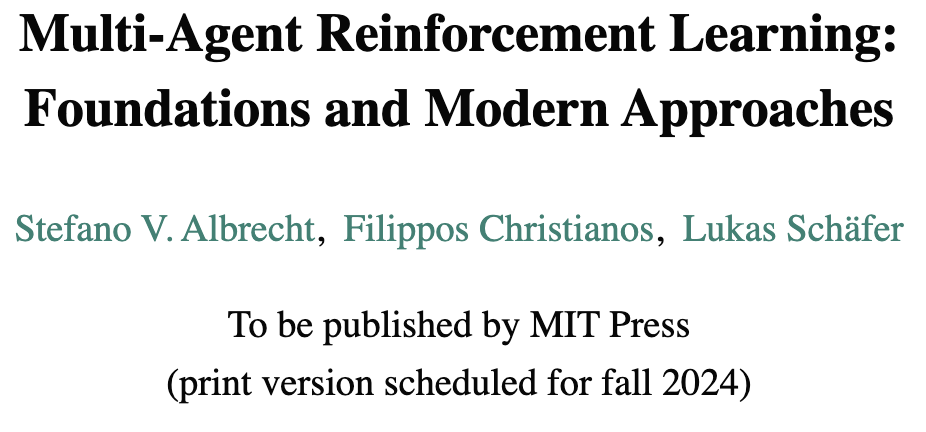
\includegraphics[width=\textwidth,height=.8\textheight,keepaspectratio]{images/1_MARL_book.png}
            
              \label{fig:enter-label}
            \end{figure}
          \end{column}
        
        \hspace{20pt}
            
          % Column for the text
            \begin{column}{0.45\textwidth}
	        \small

                This lecture is based on \textit{Multi-Agent Reinforcement Learning: Foundations and Modern Approaches} by Stefano V. Albrecht, Filippos Christianos and Lukas Sch\"afer
                
                \vspace{20pt}
                
                The book can be downloaded for free at \textcolor{blue}{\href{https://www.marl-book.com/}{www.marl-book.com}}.
            \end{column}
        
        \end{columns}
    \end{frame}
}

\newcommand{\leoslide}{
  \author{Stefano V. Albrecht, Filippos Christianos, Lukas Sch\"afer \\ Slides by: Leonard Hinckeldey}
}

\newcommand{\otherslide}{
  \author{Stefano V. Albrecht, Filippos Christianos, Lukas Sch\"afer}
}
	
\title{Multi-Agent Reinforcement Learning}
\date{}

\hypersetup{
  pdfsubject = {Multi-Agent Reinforcement Learning},
}

\leoslide

\subtitle{Deep Learning}

\begin{document}
\maketitle

\introslide

\begin{frame}{\outline}

\blist
    \item Function approximation 
    \item Feed forward neural networks
    \item Training neural networks
    \item Additional neural network architectures
\elist
    
\end{frame}

\section{Function Approximation}

\begin{frame}[t]{Motivation for Function Approximation in RL}

\begin{problembox}
    Previously introduced RL and MARL algorithms maintain \fat{tabular} value functions with a value for each state-action pair. \pause This has 2 major limitations:

    \begin{enumerate}
        \item<2-> The table grows linearly with the number of possible inputs \pause $\rightarrow$ difficult in complex environments (e.g., Go has approximately $10^{170}$ possible states)
        \item<4-> Each value is updated in isolation \pause\pause $\rightarrow$ agents need to visit each state-action pair to obtain accurate values
    \end{enumerate}
    \vspace{-.5em}
\end{problembox}

\visible<6->{
    \begin{solutionbox}
        We need value functions that \fat{generalise} across inputs.
    \end{solutionbox}
}
\end{frame}

\begin{frame}{Generalization}

\begin{columns}
    \begin{column}{0.4\textwidth}
        \begin{figure}
            \centering
            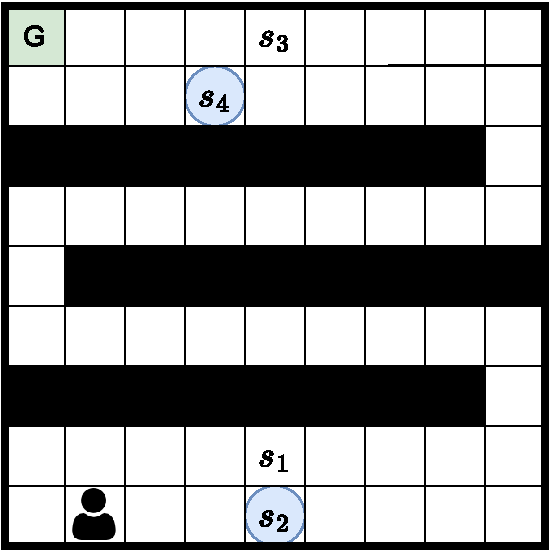
\includegraphics[width = 0.9\textwidth, keepaspectratio]{images/chapter_7/maze.pdf}
        \end{figure}
    \end{column}
    \begin{column}{0.6\textwidth}
        \blist
            \item The agent must reach the goal location (G)
            \item The agent has already seen states $s_1$ and $s_3$ during past trajectories, but not $s_2$ and $s_4$
            \item States $s_2$ and $s_4$ are similar to $s_1$ and $s_3$ respectively
            \item It would be beneficial if the agent could generalize from $s_1$ and $s_3$ to estimate the values of $s_2$ and $s_4$
        \elist 
    \end{column}
\end{columns}
\end{frame}

\begin{frame}{Function Approximation}

Function approximation is one way to find generalizable representations for value functions. 

\blist
\item Function approximations learns a \fat{parameterized} function $f(x; \theta)$ for some input $x \in \mathbb{R}^{d_x}$ such that: 
\elist
\vspace{-2pt}
\[
\forall x: f(x; \theta) \approx f^*(x)
\]

\blist
    \item Training a function approximator involves optimizing the parameters $\theta$ such that $f$ accurately \fat{approximates} $f^*$
    \item In RL $f^*$ might be the true value function of the environment representing the expected return given as state $s$ as input
\elist

    
\end{frame}

\begin{frame}[t]{Linear Function Approximation}

One approach for function approximation is to represent $f(x; \theta)$ as a linear function. For instance, a linear state-value function:

\[
\hat{V}(s; \theta) = \theta^\top x(s) = \sum^d_{k=1}\theta_k x_k (s)
\]

\blist
    \item $x(s)$ denotes the state feature vector
    \item We can then optimize the parameters using a \fat{loss function} like mean square error
\elist

% \only<1>{
% \[
% \theta^* = \arg \min_\theta \mathbb{E}_{s \in S}\left[(V^\pi (s) - \hat{V}(s; \theta))^2 \right]
% \]
% }

% \only<1>{\blist
%     \item We can find optimal $\theta$ values by computing gradients of all $\theta_i \in \theta$ with respect to the loss and \fat{descent} along the gradient
%     \item With optimal parameters $\hat{V}(s; \theta)$ might be close to the true value function, allowing us to estimate values by 'plugging in' new potentially unseen states
%     \item 
% \elist 
% }

\only<2->{
    \begin{notebox}
        The function is \fat{linear} in \fat{parameters} but we can transform the input features $x(s)$ to approximate non-linear value functions e.g. $x(s^2)$ for quadratic functions   
    \end{notebox}
}

\end{frame}

\begin{frame}[t]{Linear Function Approximation Optimization}

We might optimize $f(x; \theta)$ using a \fat{mean squared error} loss.

\[
\theta^* = \arg \min_\theta \mathbb{E}_{s \in S}\left[(V^\pi (s) - \hat{V}(s; \theta))^2 \right]
\]

\blist
    \item<2-> We can find optimal $\theta$ values by computing gradients of all $\theta_i \in \theta$ with respect to the loss and descend along the gradient
\elist
\only<2>{
    \vspace{-1.3em}
    \begin{figure}
        \centering
        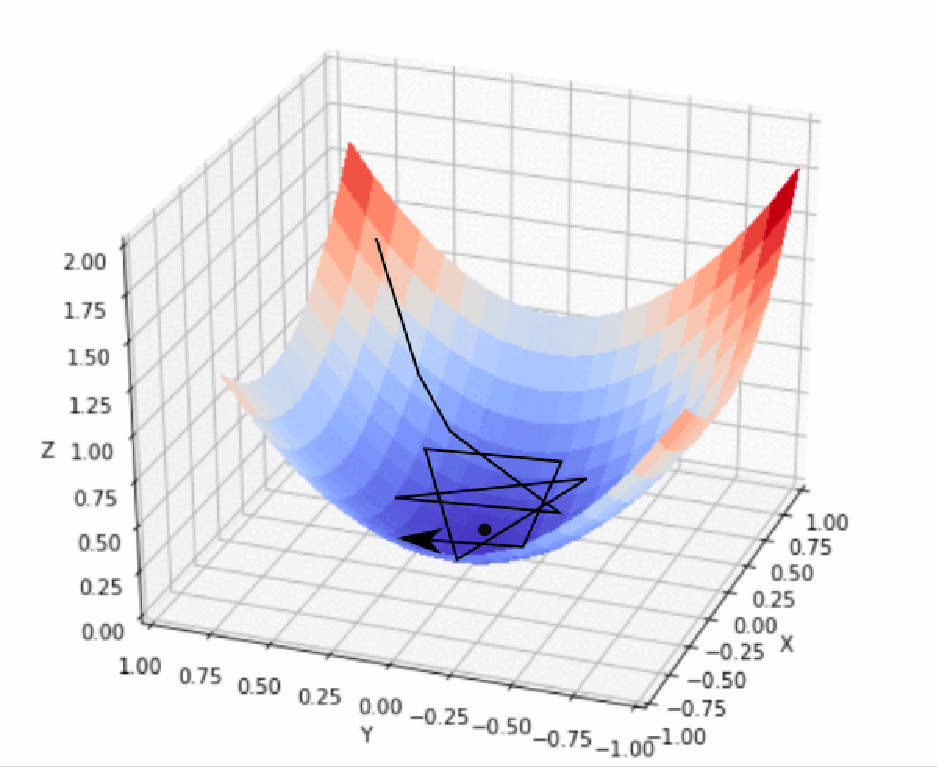
\includegraphics[height=0.5\textheight, keepaspectratio]{images/chapter_7/sgd.pdf}
        % \caption{Caption}
        % \label{fig:enter-label}
    \end{figure}
}
\blist
    \item<3-> With optimal parameters $\hat{V}(s; \theta^*)$ might be close to the true value function, allowing us to estimate values by 'plugging in' new potentially unseen states
    \item<4-> Linear function approximation is a simple and powerful way to find generalizable functions
\elist

\end{frame}

% \begin{frame}{Deep Learning for Function Approximation}

% Linear functions are a powerful way to find generalisable functions, but they depend on finding good feature representations. In contrast, deep learning can learn feature representations automatically.

% \blist
%     \item Deep learning encompasses a family of machine learning techniques that apply \fat{neural networks} as function approximators
%     \item Neural networks consist of:
%     \begin{itemize}
%         \item Sequential \textbf{layers}
%         \item Layers consist of \textbf{neural units}
%         \item Neural units are interconnected across layers by \textbf{parameters }(weights and biases) 
%         \item Neural units compute \textbf{activations} which are simple \textbf{non-linear transformation} of their inputs
%     \end{itemize}
% \elist
    
% \end{frame}

\begin{frame}[t]{Deep Learning for Function Approximation}

 The main benefit of linear value functions is their simplicity and generalization ability. However, linear function approximation heavily relies on the selection of state features.


\textbf{Deep Learning Advantages:}
\blist
    \item Universal method, leveraging \fat{neural networks} for function approximation
    \item Automatically learns feature representations of states
    \item Able to represent non-linear, complex functions
    \item Is effective with high-dimensional data such as images and text
\elist
    
\end{frame}

\section{Neural Networks}

\begin{frame}[t]{Feedforward Neural Networks}

\e{Feedforward neural networks}, fully-connected neural networks, or multi-layer perceptrons can be considered as the building block of most neural networks.

\only<1>{
\begin{figure}
    \centering
    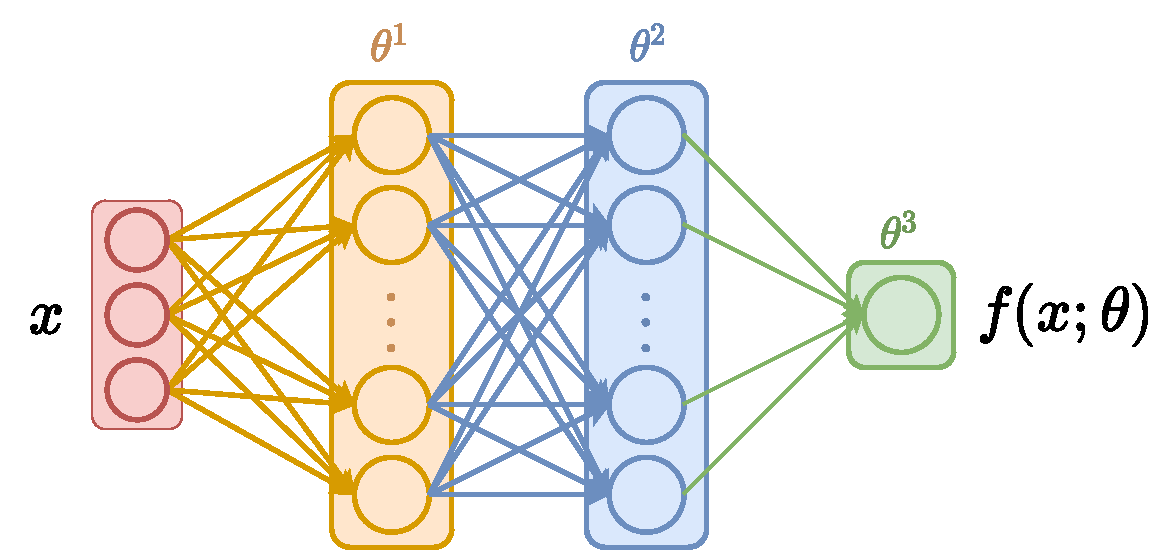
\includegraphics[width=0.7\textwidth, keepaspectratio]{images/chapter_7/feedforward_neural_network.pdf}
\end{figure}
}

\vspace{10pt}
\begin{columns}
    \begin{column}{0.4\textwidth}
    \only<2->{
    \begin{figure}
    \centering
    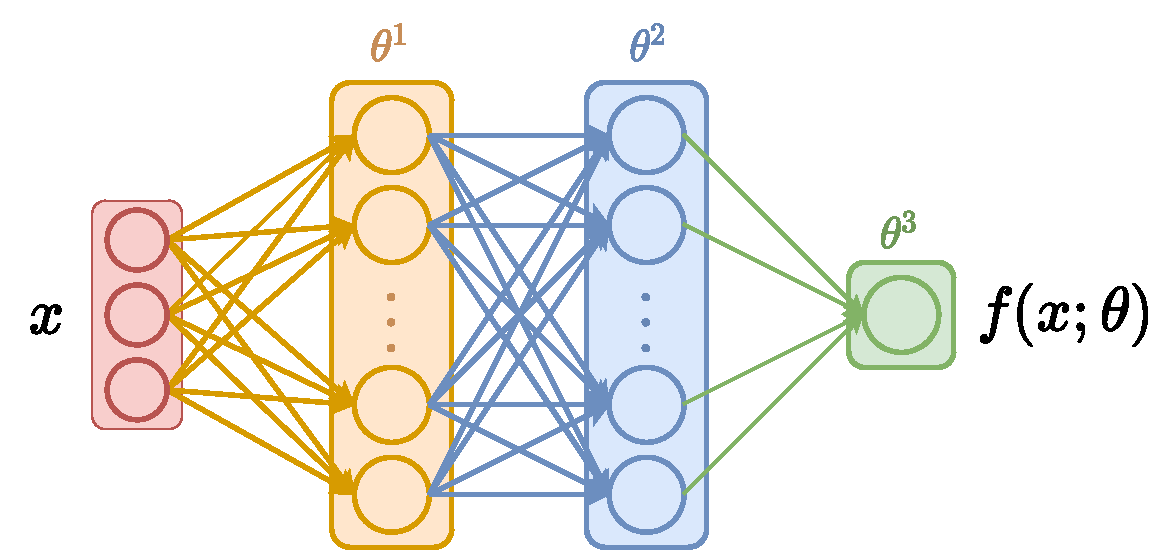
\includegraphics[width=\textwidth, keepaspectratio]{images/chapter_7/feedforward_neural_network.pdf}
    \end{figure}
    }
    \end{column}
    \begin{column}{0.6\textwidth}
        \only<2>{
        \blist
            \item A feedforward NN consists of multiple sequential layers
            \item The first layer processes input $x$, subsequent layers process the outputs of previous layers
            \item Each layer is defined as a parameterized function and is composed of many neural units
            \item We typically refer to the first layer as the \fat{input layer} and the last layer as the \fat{output layer} and all layers in between as \fat{hidden layers}
        \elist
        }
         \only<3->{

    \begin{blackbox}
        Mathematically, this can be represented as a compositional function:

        \[
        f(x; \theta) = (f_2(f_1(x; \theta^1); \theta^2))
        \]

        where $f_k$ corresponds to the function of layer $k$ with parameters $\theta^k$ 
    \end{blackbox}
    }
    \end{column}
\end{columns}
    
\end{frame}

% \begin{frame}{Universal Functin Approximation}


    
% \end{frame}

\begin{frame}[t]{Neural Unit}

An individual unit of a neural network in layer $k$ represents a parameterized function $f_{k, u}: \mathbb{R}^{d_{k-1}} \to \mathbb{R}$ which processes the output of the previous layer. 

\only<1>{
\begin{figure}
    \centering
    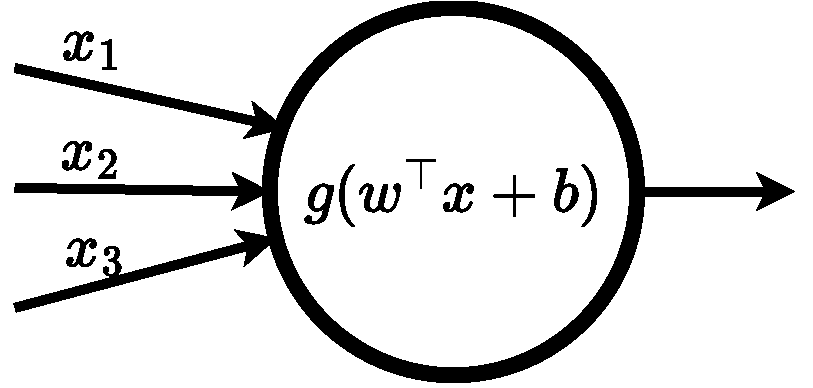
\includegraphics[width = 0.7\textwidth, keepaspectratio]{images/chapter_7/neural_unit.pdf}
\end{figure}
}

\vspace{5pt}
\begin{columns}
    \begin{column}{0.5\textwidth}
    \only<2->{
    \blist
        \item The previous layer's output is the concatenation of all its units' outputs
        \item Formally this is:
    \elist
    \[
    f_{k, u}(x; \theta^k_u) = g_k(w^\top x + b)
    \]
    \blist
        \item $\theta_u^k$ is the weight vector $w$ as well as the scalar bias $b$
        \item $g_k$ is a \fat{non-linear} activation function 
    \elist
    }
        
    \end{column}
    \begin{column}{0.5\textwidth}
    \only<2>{
    \begin{figure}
        \centering
        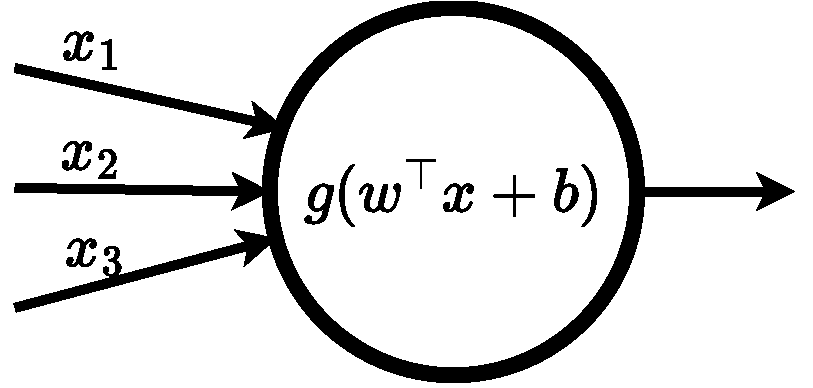
\includegraphics[width = 0.9\textwidth, keepaspectratio]{images/chapter_7/neural_unit.pdf}
    \end{figure}
    }
    \only<3->{
    \begin{notebox}
        Applying a \fat{non-linear} activation function is essential, because the composition of two linear function $f$ and $g$ can only represent a linear function itself.     
\end{notebox}
    }
    \end{column}
\end{columns}    
\end{frame}

\begin{frame}{Activation Functions}

\begin{figure}
    \centering
    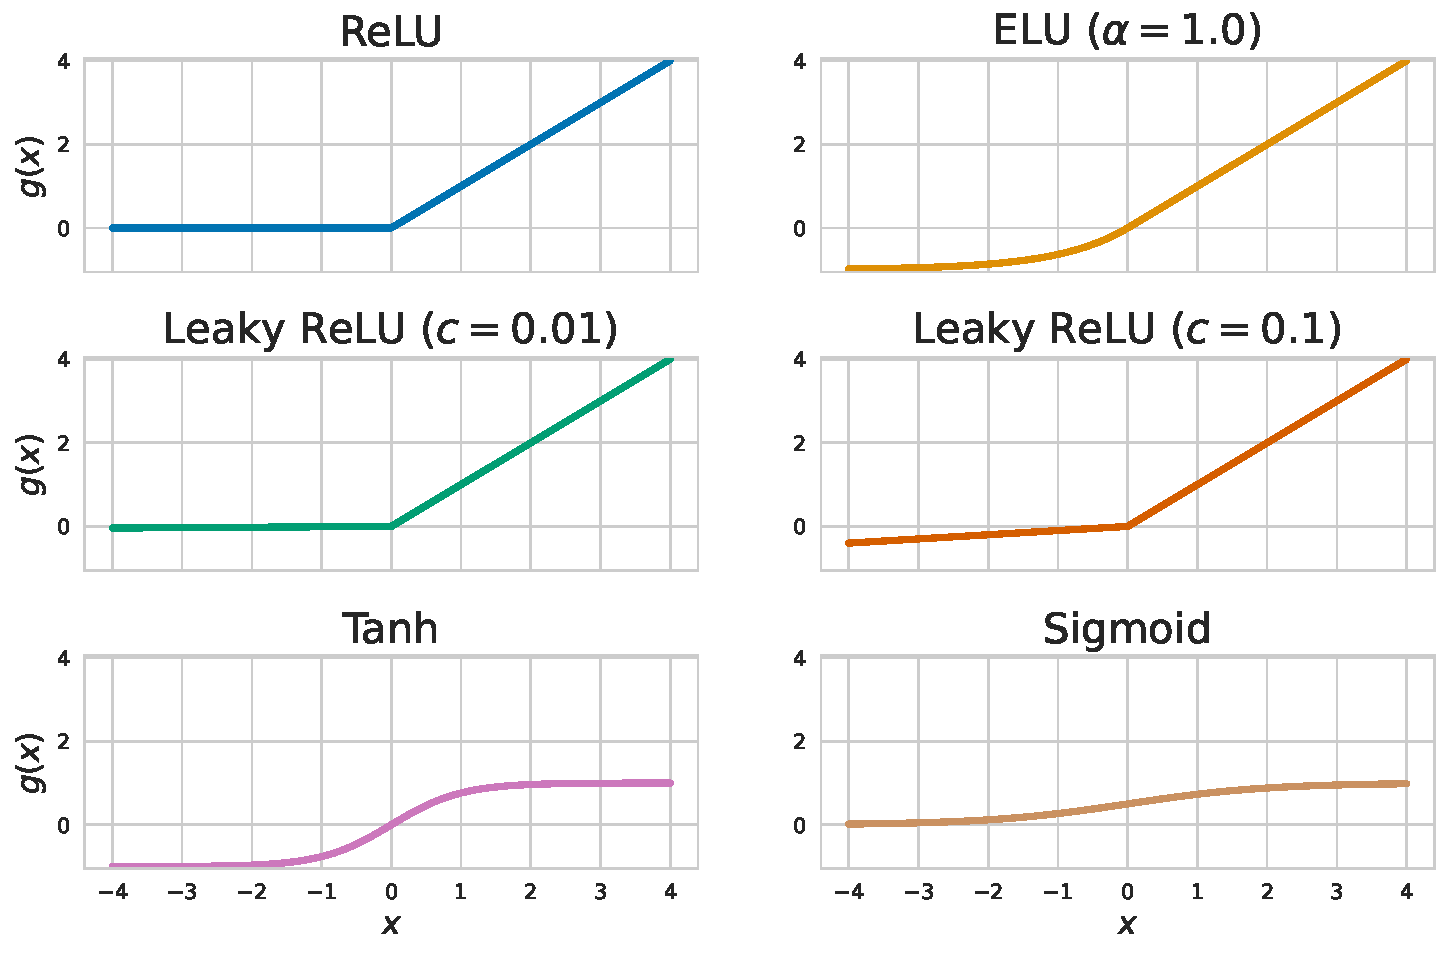
\includegraphics[width = 0.8\textwidth, keepaspectratio]{images/chapter_7/activation_functions.pdf}
    \end{figure}
\end{frame}

\begin{frame}[t]{Computation of Neural Network Layer}

We can use vector notation to aggregate the computation of all neural units of layer $k$ as:
\vspace{0pt}
\[
f_k(x_{k-1}; \theta^k) = g_k(W_k^\top x_{k-1} + b_k)
\]

\blist
    \item $W_k \in \mathbb{R}^{d_{k-1} \times d_k}$ is a weight matrix
    \item $b_k \in \mathbb{R}^{d_k}$ is the bias vector
\elist

The high-dimensional linear transformation of a single layer $k$ can now be described as a single matrix multiplication with $W_k$, followed by vector addition with $b_k$ and applying an activation function $g_k$ element-wise, resulting in an output vector.
    
\end{frame}

\begin{frame}[t]{Universal Function Approximation Theory}

The \fat{universal function approximation theory} states that with as little as one hidden layer, a feedforward neural network can approximate \fat{any} function. 
\vspace{3pt}
\blist
    \item This theory assumes arbitrary \fat{width} of the hidden layer
    \item We refer to the number of neural units within hidden layers as the \fat{width} of the network
    \item The number of layers is referred to as the \fat{depth}
    \item In practice, \fat{deep} neural networks can outperform shallow ones and in some cases, require fewer parameters to do so
\elist
    
\end{frame}

\section{Training Neural Networks}

\begin{frame}[t]{Gradient Based Optimization}

To train a neural network, we repeatedly update the parameters $\theta$ such that $f(x; \theta)$ becomes better at approximating a target function. 

\only<1>{
\begin{figure}
    \centering
    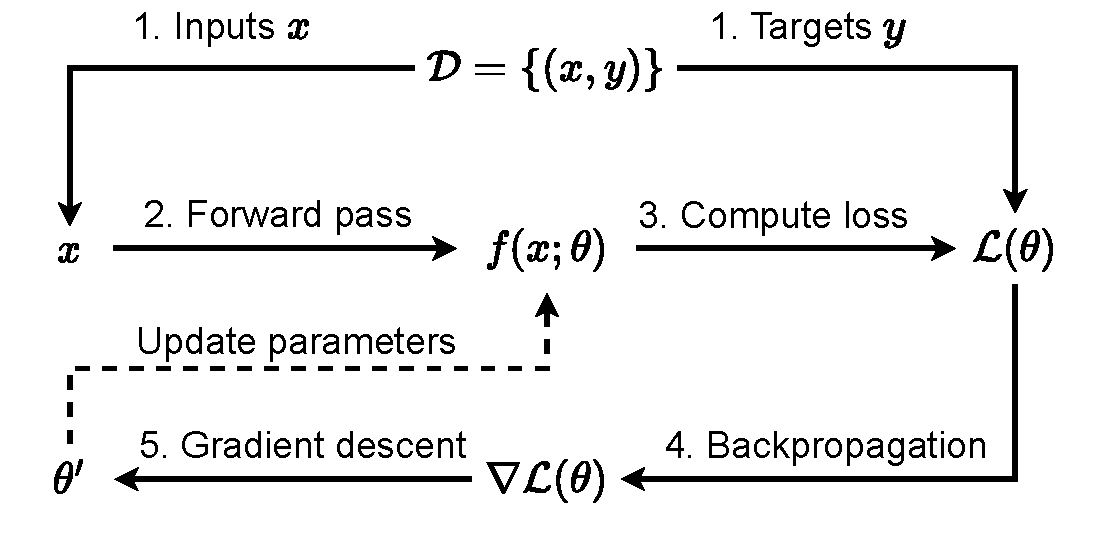
\includegraphics[width = 0.7\textwidth, keepaspectratio]{images/chapter_7/dl_training_loop.pdf}
\end{figure}
}

\vspace{10pt}
\begin{columns}
    \begin{column}{0.5\textwidth}
    \visible<2->{
        \begin{figure}
            \centering
            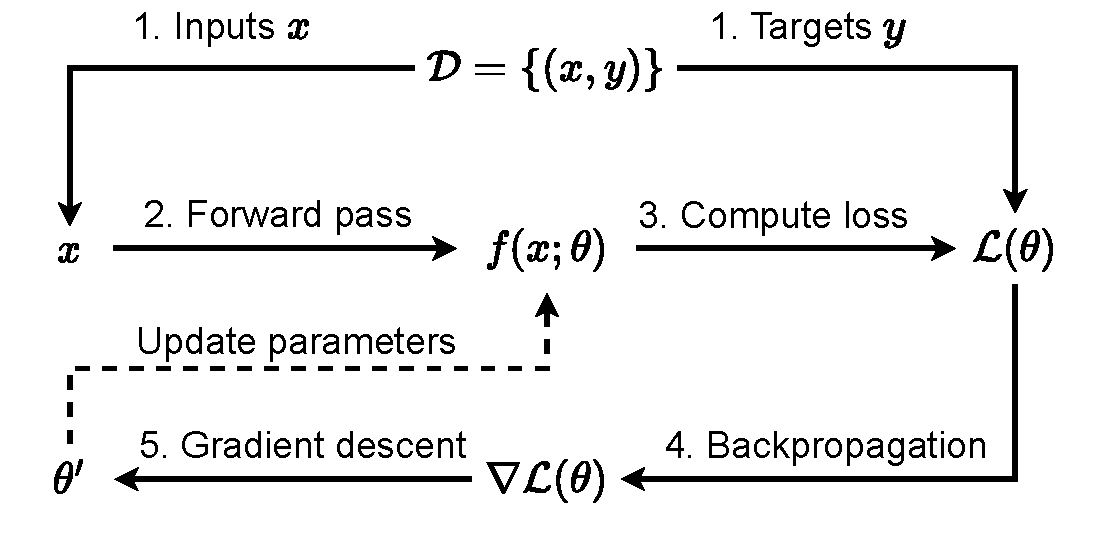
\includegraphics[width=\textwidth, keepaspectratio]{images/chapter_7/dl_training_loop.pdf}
        \end{figure}
    }
    \end{column}
    \begin{column}{0.5\textwidth}
        \visible<2->{
            Steps of the optimization process
            \begin{enumerate}
                \item Gather batch of input-target $(x,y)$ pairs
                \item Compute network output for given inputs $f(x; \theta)$
                \item Compute the loss over network outputs and targets $y$
                \item Backpropagation (compute gradients)
                \item Gradient descent (update $\theta$)
            \end{enumerate}
        }
    \end{column}
\end{columns}
    
\end{frame}

\begin{frame}[t]{Loss Function}

The loss function indicates how 'wrong' the neural network estimates are. In optimization the objective is to find $\theta$ such that the loss is minimized:\\ \begin{center}$\theta^* \in \arg \min_{\theta} \mathcal{L}(\theta)$\end{center}

\vspace{0pt}
\only<2->{\blist
    \item Knowing the true values (supervised learning) allows us to construct a loss by comparing the neural network estimated value with the true value, e.g., MSE:
\elist
\vspace{0pt}
\[
\mathcal{L}(\theta) = \frac{1}{B} \sum_{k =1}^B (V^\pi(s_k) - \widehat{V}(s_k ; \theta))^2
\]}

\only<2>{\blist
    \item Where $\mathcal{B}$ is a \fat{batch} ($B$ is batch size) of states and true value $V^\pi(s_k)$ pairs
    \item Minimizing the loss leads to parameters $\theta$ such that $\widehat{V}(s_k; \theta)$ more accurately approximates the true value function
\elist}

\only<3->{
    \begin{orangebox}
        Minimizing the loss will optimize $\theta$ such that $\widehat{V}$ will gradually provide more accurate state-value estimates.
\end{orangebox}
}

\end{frame}

\begin{frame}{Gradient Descent}

Gradient descent sequentially updates the parameters $\theta$ by following the \fat{negative} (hence "descent") \fat{gradients} of the loss function with respect to the parameters for given data.

\only<1>{
\begin{figure}
    \centering
    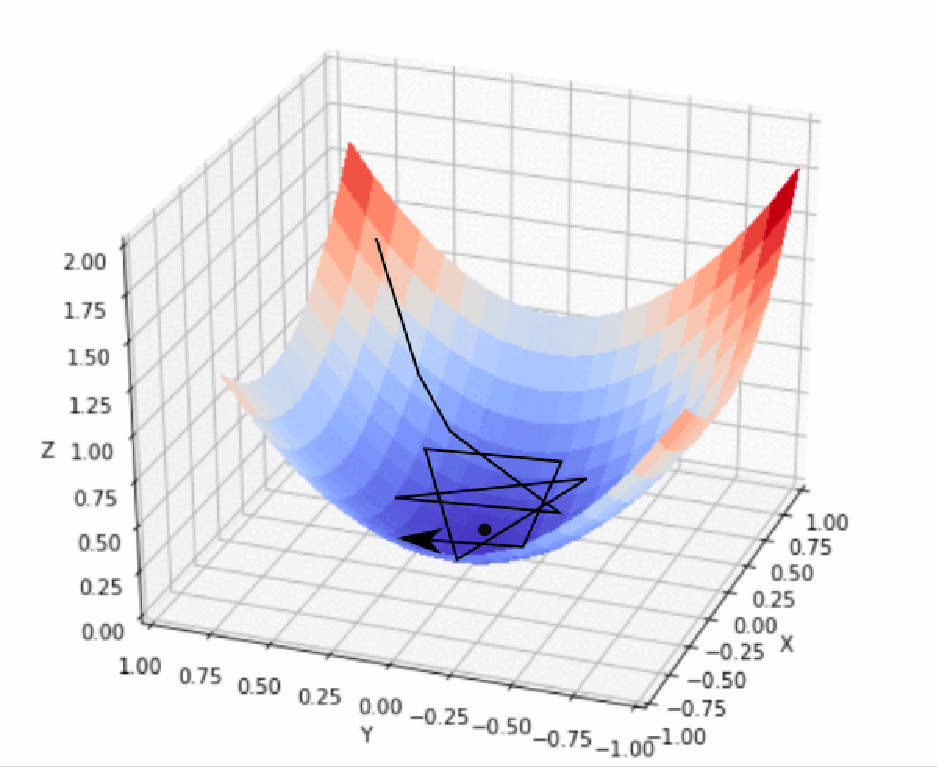
\includegraphics[height=0.6\textheight, keepaspectratio]{images/chapter_7/sgd.pdf}
    % \caption{Caption}
    % \label{fig:enter-label}
\end{figure}
}


\only<2->{
\blist 
    \item The gradient is defined as a \fat{vector} of partial derivatives one for each $\theta_i \in \theta$
\elist
\vspace{0pt}
\[
 \nabla\mathcal{L}(\theta) = \left(\frac{\partial\mathcal{L}(\theta)}{\partial\theta_1}, \dots,\frac{\partial\mathcal{L}(\theta)}{\partial\theta_d} \right)
\]

\blist 
    \item In the simplest case, gradient descent updates the parameters as follows:
\elist
\vspace{0pt}
\[
\theta \leftarrow \theta - \alpha \nabla_\theta \mathcal{L}(\theta \mid \mathcal{D})
\]

\blist 
    \item $\alpha$ is the learning rate and $\mathcal{D}$ the training data
\elist
}

\end{frame}

\begin{frame}[t]{Stochastic Gradient Descent}

\begin{problembox}
    The application of (vanilla) gradient descent has some downsides:
    \blist
        \item Computing gradients across the entire dataset $\mathcal{D}$ is costly (often doesn't fit in memory)
        \item Convergence is slow due to computational overhead of computing gradients
    \elist
    \vspace{-1em}
\end{problembox}
\begin{solutionbox}
    \fat{Stochastic gradient descent} (SGD) instead computes gradients over randomly sampled data pairs $d \sim \mathcal{U(\mathcal{D})}$ (speeds up convergence but increases variance): 
    \begin{equation*}
        \theta \leftarrow \theta - \alpha \nabla_\theta \mathcal{L}(\theta \mid d)\lvert_{d \sim \mathcal{U(\mathcal{D})}}
    \end{equation*}
\end{solutionbox}
    
\end{frame}

\begin{frame}[t]{Mini-batch Gradient Descent}

    Mini-batch gradient descent is a middle ground between SGD and GD.

    \blist
        \item Randomly samples a predefined \fat{batch} of data pairs 
        \item This reduces variance compared to SGD while still converging much faster than GD
    \elist
    \vspace{0pt}
    \[
    \theta \leftarrow \theta - \alpha \nabla_\theta \mathcal{L}(\theta|\mathcal{B})|_{\mathcal{B} = \{d_i \sim \mathcal{U(\mathcal{D})}\}^B_{i=1}}
    \]

    \blist
        \item $\mathcal{B}$ denotes a \fat{batch} and the \fat{batch size} is a hyperparameter determined by $B$
        \item The \fat{batch size} can be adjusted depending on the computational power available and the type of data being worked with
    \elist
    
\end{frame}

\begin{frame}{GD vs SGD vs MGD}

\begin{minipage}{.6\textwidth}
    \begin{figure}
        \centering
        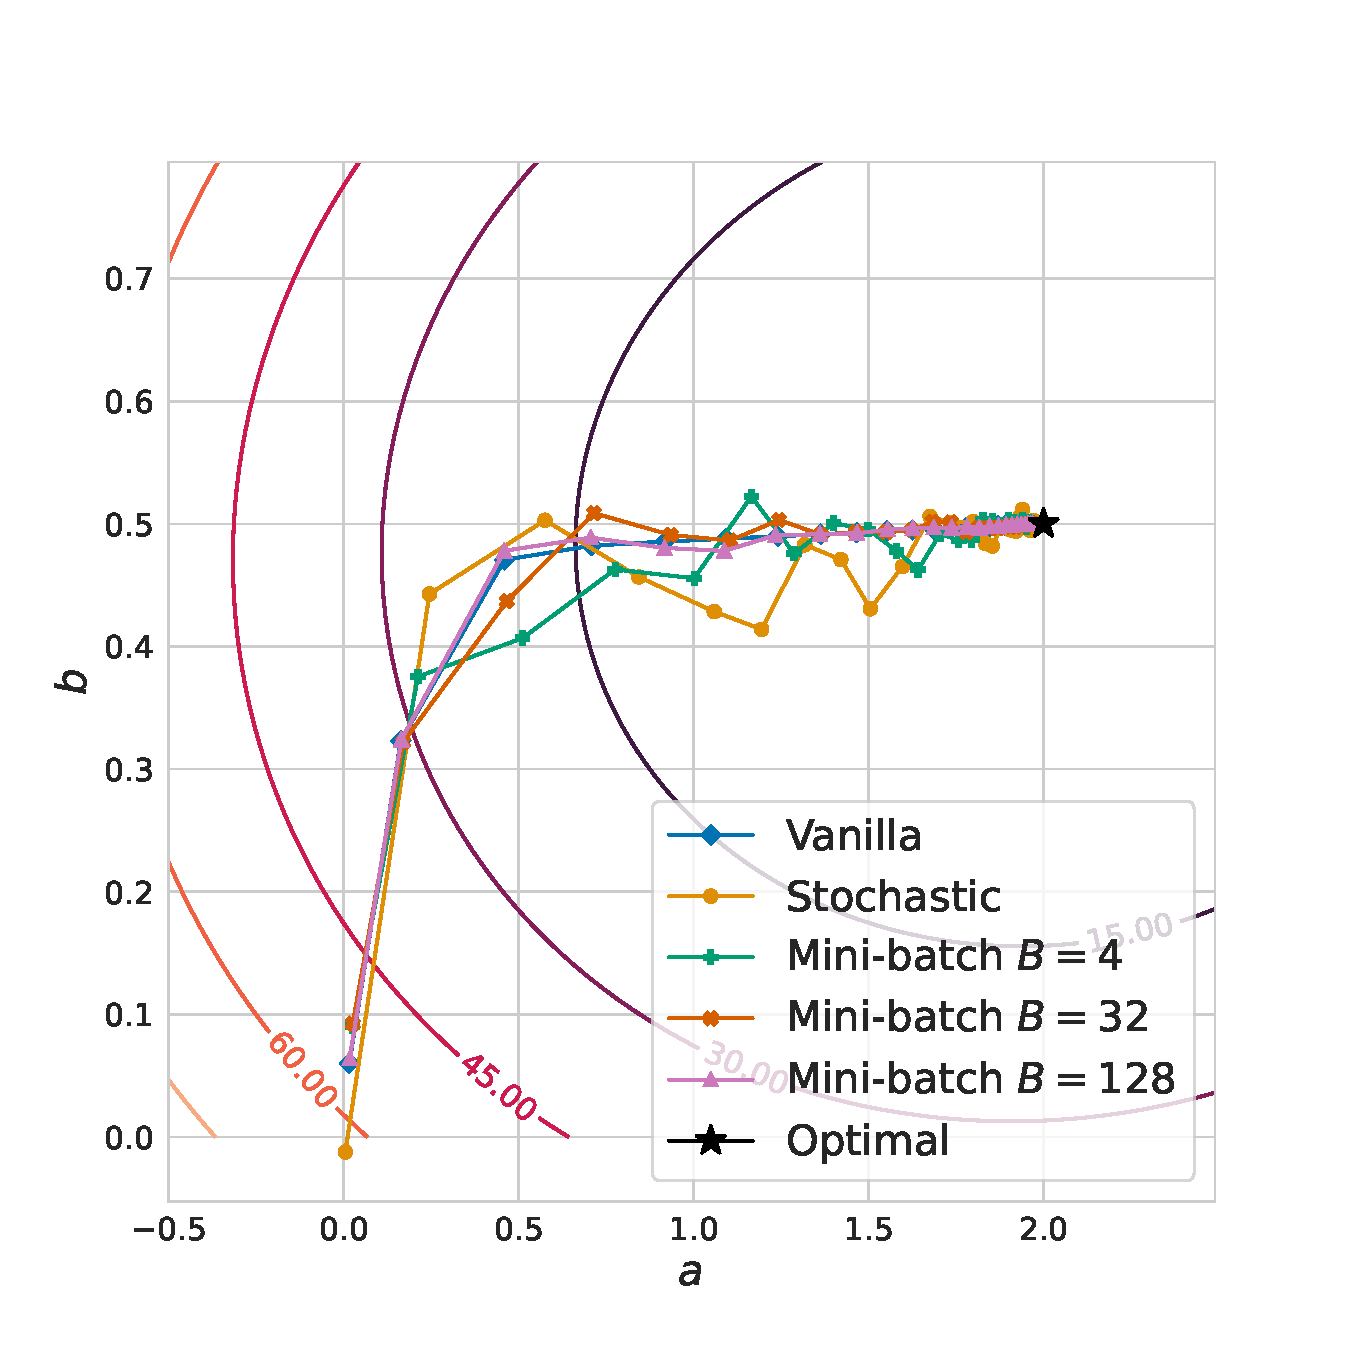
\includegraphics[width=0.9\textwidth]{images/chapter_7/gradient_optimisation_contour.pdf}
    \end{figure}
\end{minipage}
\begin{minipage}{.39\textwidth}
    \blist
        \item \fat{Vanilla gradient descent:} smooth optimization but each step is expensive
        \item \fat{Stochastic gradient descent:} less stable optimization but is notably faster per step
        \item \fat{Mini-batch gradient descent:} stable optimization for larger batch sizes and efficient
    \elist
\end{minipage}
    
\end{frame}

\begin{frame}{Momentum}

Modern optimization algorithms often also use \fat{momentum}.

\begin{columns}
    \begin{column}{0.5\textwidth}
        \begin{figure}
            \centering
            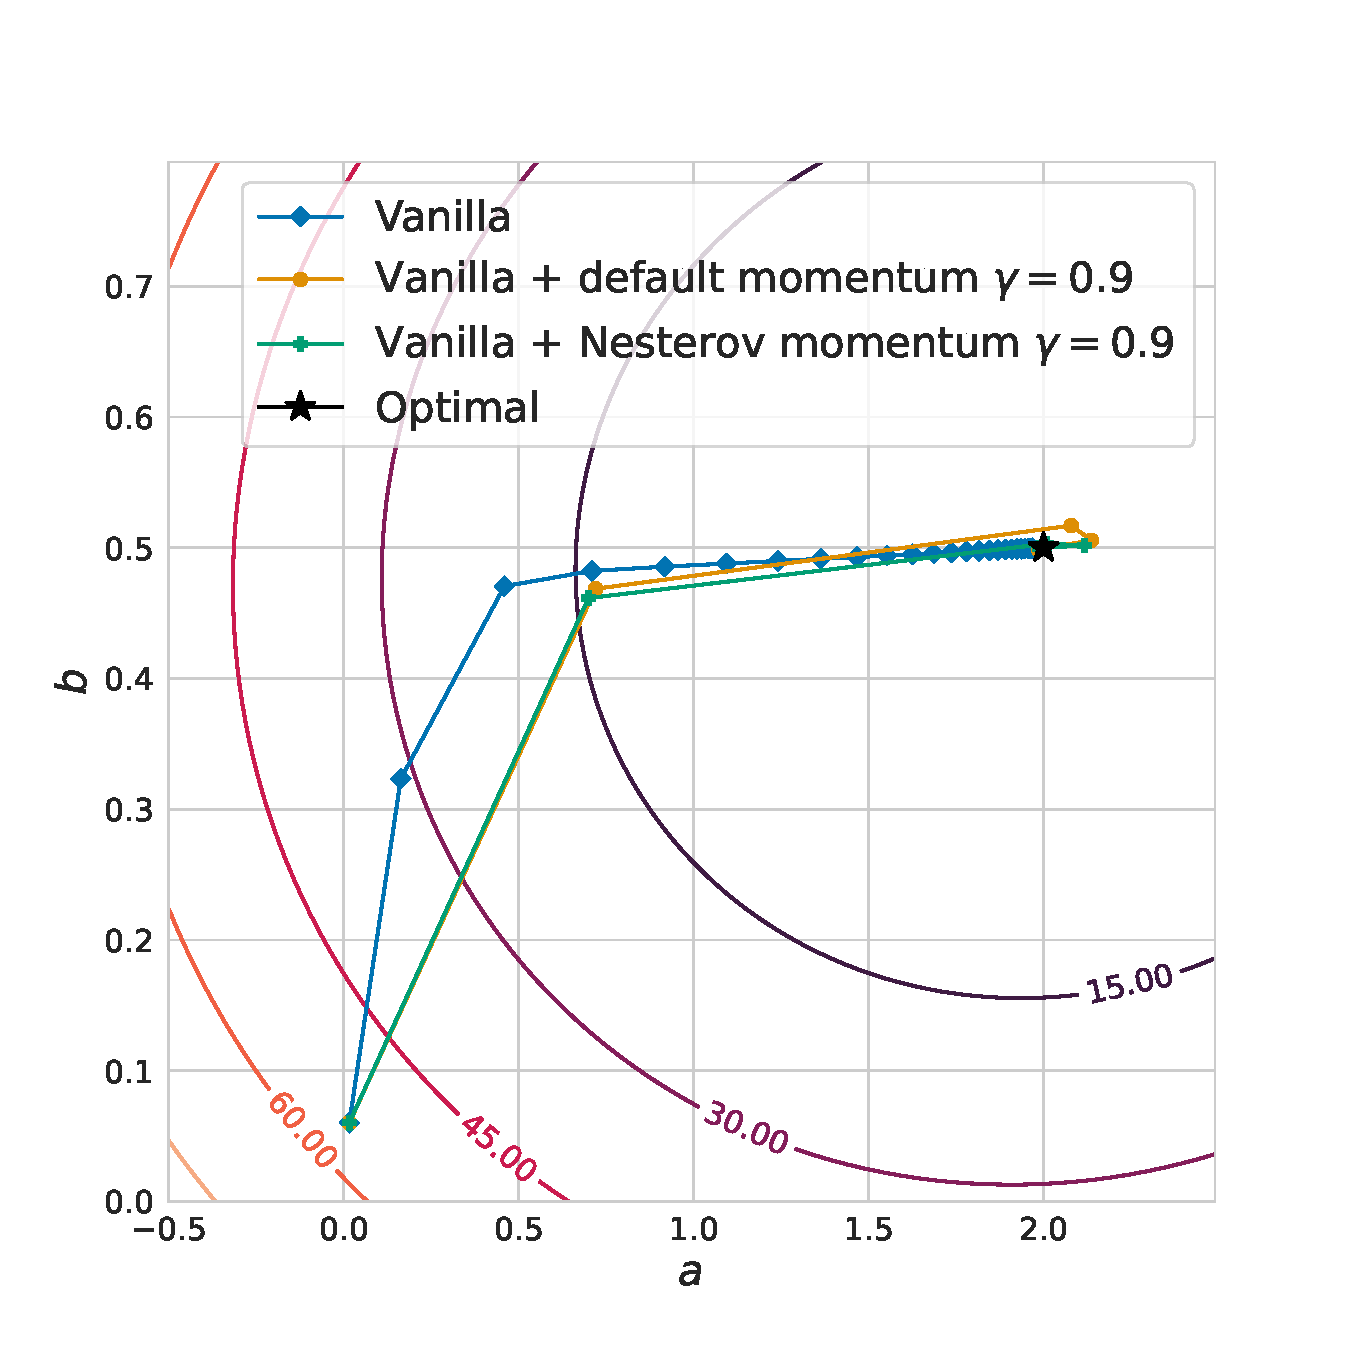
\includegraphics[width=0.9\textwidth]{images/chapter_7/gradient_optimisation_momentum_contour.pdf}
        \end{figure}
    \end{column}
    \begin{column}{0.5\textwidth}
    \blist
        \item \fat{Momentum} computes moving averages over past gradients to "accelerate" convergence
        \item This works particularly well if gradients consistently follow a similar direction
        \item There are more recent optimisers which also dynamically adjust the learning rate; one popular such optimiser is \fat{Adam} (Kingma and Ba 2015)
        
    \elist
    \end{column}
\end{columns}
    
\end{frame}

\begin{frame}[t]{Backpropagation}

Backpropagation is the algorithm that computes the gradients for \fat{every} parameter in the neural network. 

\blist
    \item The algorithm applies the \fat{chain rule} making use of the compositional function of the neural network (i.e. $f(x; \theta) = f_2(f_1(x; \theta^1);\theta^2)$)
\elist

\only<1>{
    \begin{reminderbox}
        The chain rule states that for $y = g(x)$ and $z = f(y)= f(g(x))$:
        \[
        \nabla_x z = \left(\frac{\partial y}{\partial x}\right)^\top \nabla_y z 
        \]
        Here $\frac{\partial y}{\partial x}$ is the Jacobian matrix of function $g$.
    \end{reminderbox}
}

\begin{columns}
    \begin{column}[b]{0.3\textwidth}
       \only<2->{\[
        \nabla_x z = \left(\frac{\partial y}{\partial x}\right)^\top \nabla_y z 
        \]}
    \end{column}
    \begin{column}{0.7\textwidth}
        \only<2->{
        \blist
        \item To efficiently find all of the gradients, we start at the output layer and traverse the network backwards layer by layer, applying the chain rule
        \item This \fat{backward pass} propagates all the gradients through the entire network
        \item These gradients are then used in \fat{gradient descent} 
        \elist}
    \end{column}
\end{columns}
    
\end{frame}


\section{Other Neural Network Architectures}

\begin{frame}[t]{Convolution and Recurrent Neural Networks }

Feedforward neural networks can, in principle, be applied to any data. There are, however, architectures designed to perform well with specific data.

Architectures often used in RL and MARL are:

\begin{enumerate}
    \item \fat{Convolutional neural networks}
    \begin{itemize}
        \item Used to process images
        \item Aims to make use of spatial correlations
        \item Often incorporate inductive biases such as invariance to local image-based translations
    \end{itemize}
        \item \fat{Recurrent neural networks}
    \begin{itemize}
        \item Used to process temporal data 
        \item Makes use of temporal correlations
    \end{itemize}
\end{enumerate}
    
\end{frame}

\begin{frame}[t]{Convolutional Neural Networks}

    \e{Convolutional neural networks} (CNNs) are neural networks for image processing
    \blist
        \item Blocks of parameters (called \fat{filters} or \fat{kernels}) are moved and repeatedly applied across an image
    \elist

    Some advantages to this architecture include:

    \blist
        \item \fat{Parameter sharing:} kernel significantly reduces the total number of parameters compared to a feedforward NN
        \item For example to process a $128 \times 128$ RGB image:
            \vspace{5pt}
        \blist
            \item Feedforward NN: input layer with $128$ hidden units has \num{6291584} parameters
            \item CNN: with sixteen $5\times5$ filters has \num{1216} parameters
        \elist
        \item \fat{Spatial correlations:} nearby pixels are likely related (e.g., edges) $\rightarrow$ same spatial patterns may occur at different locations of an image
    \elist

\end{frame}


\begin{frame}[t]{Convolutional Neural Networks}

\only<1>{\begin{figure}
    \centering
    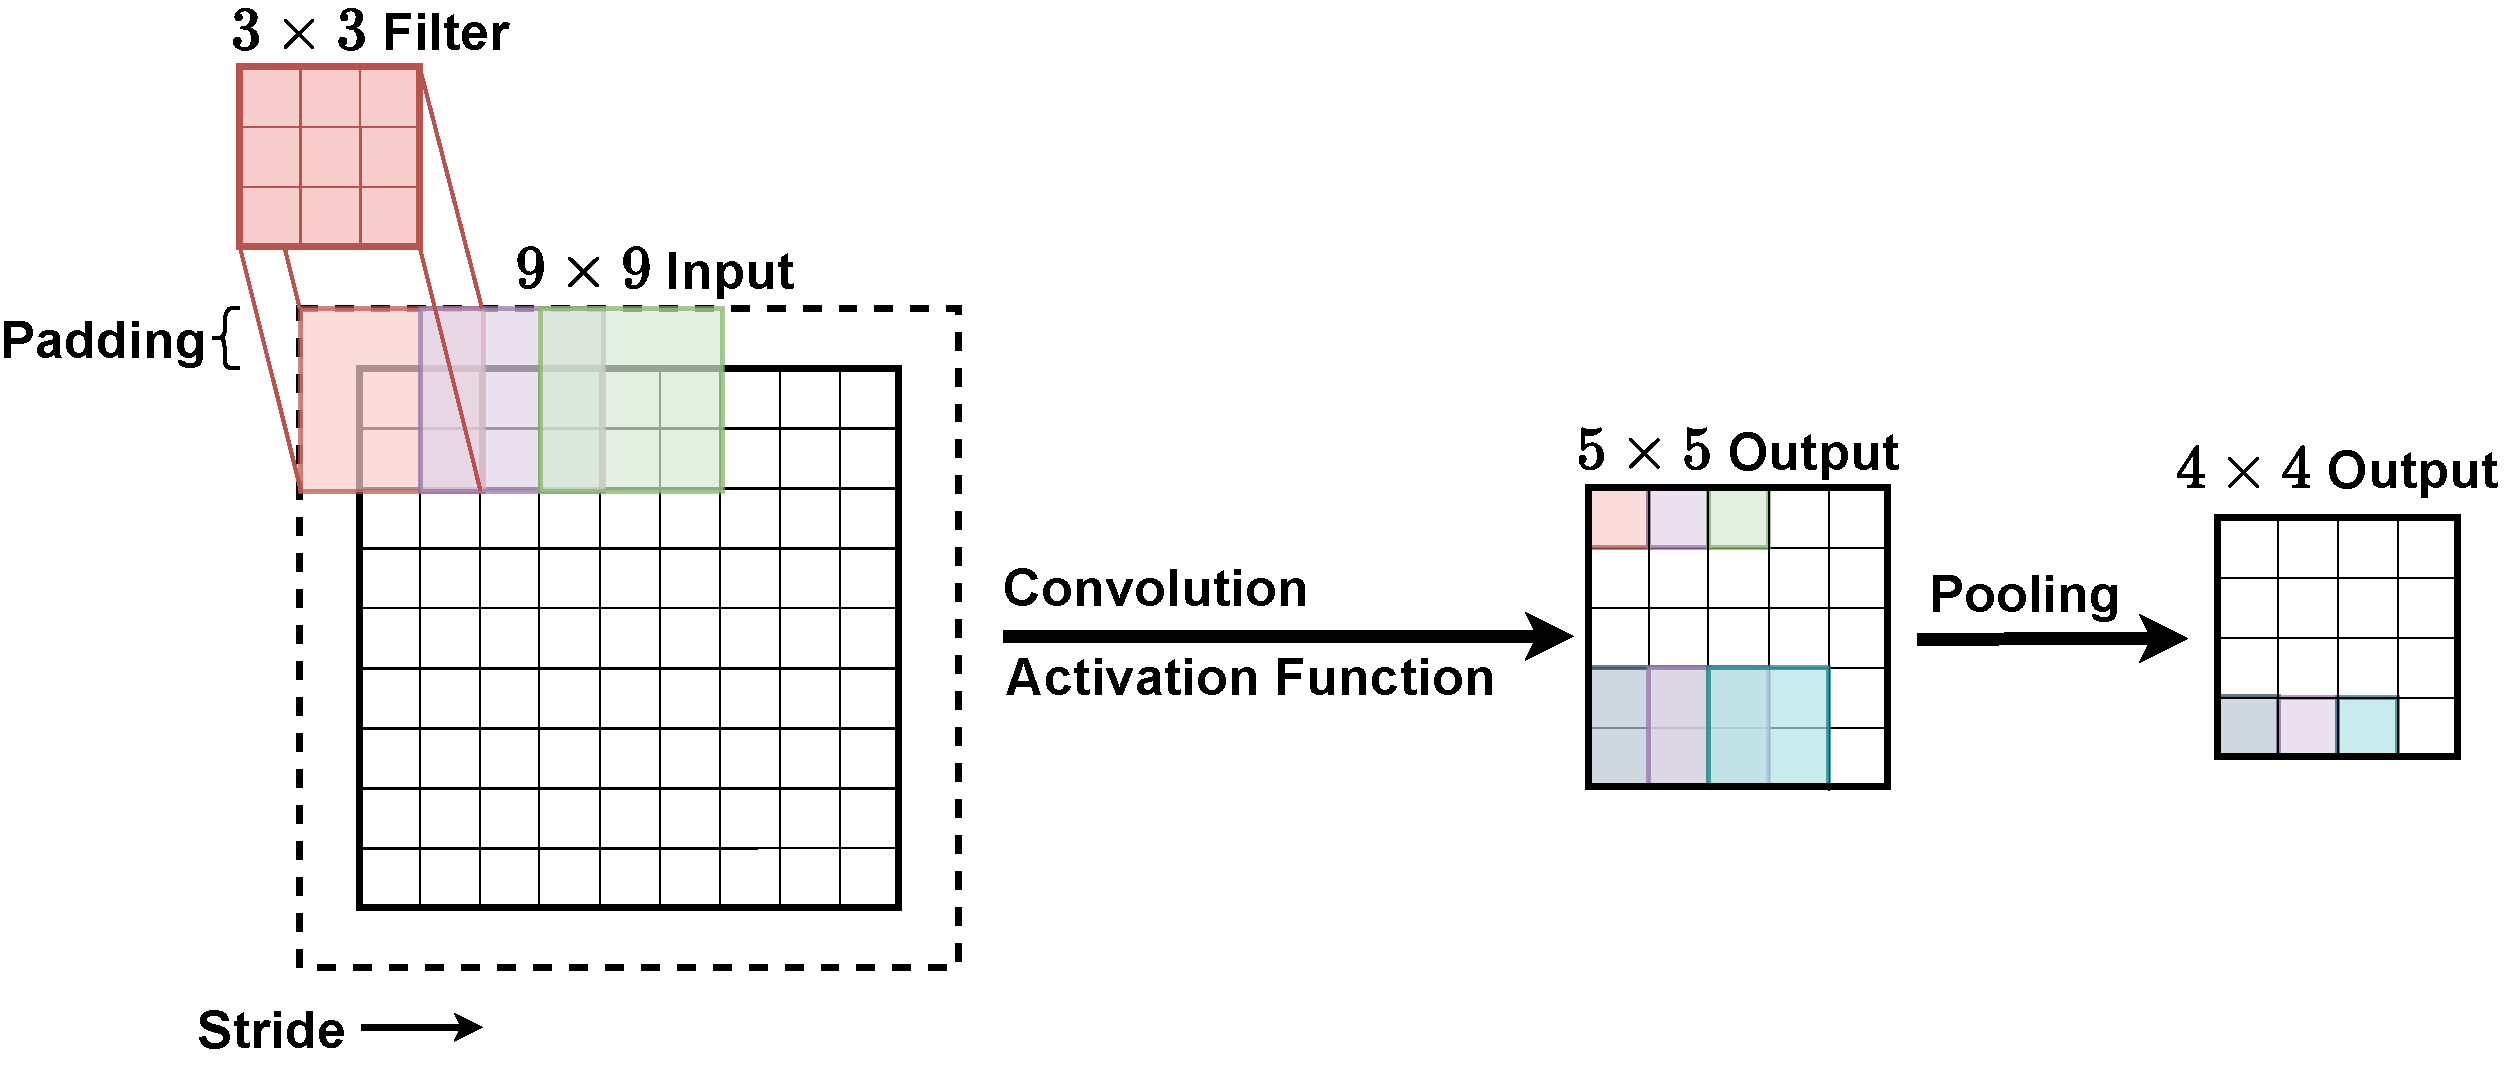
\includegraphics[width = 0.9\textwidth, height = 0.7\textheight, keepaspectratio]{images/chapter_7/cnn.pdf}
\end{figure}}

\only<2>{
\begin{figure}
    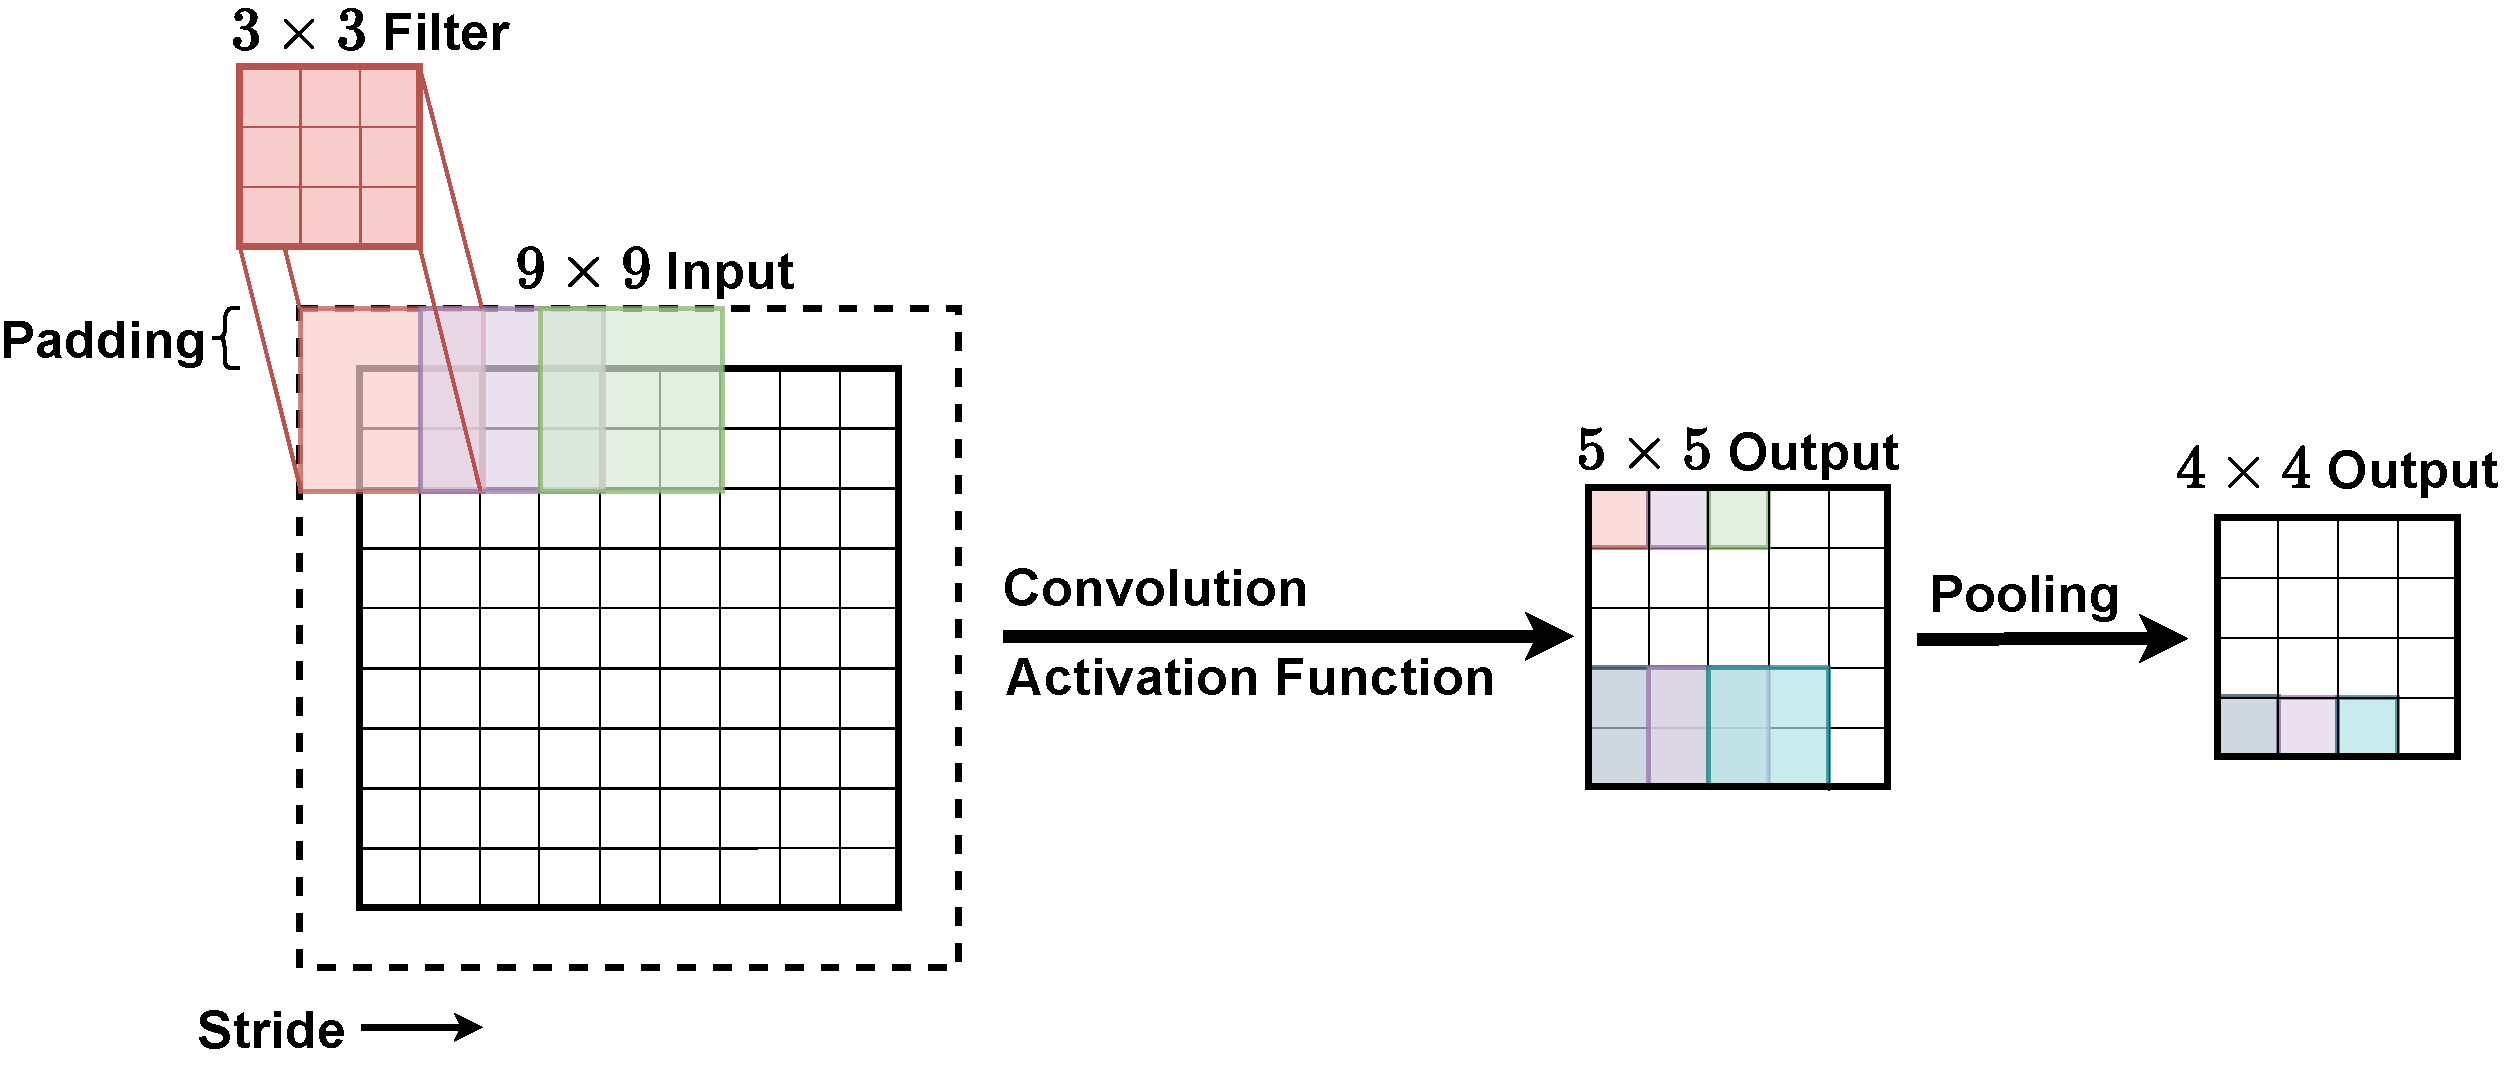
\includegraphics[width=0.5\textwidth]{images/chapter_7/cnn.pdf}
\end{figure}
}

\vspace{5pt}

\begin{minipage}{0.48\textwidth}
   \only<2->{
       \blist
            \item Filter or kernels (a collection of parameters) are moved across an image
            \item The convolution can be thought of as reducing the dimensional (e.g. taking in 3 $\times$ 3 patch of pixels and returning one single value)
            % \item A convolution of a filter with parameters $W \in \mathbb{R}^{d_w \times d_w}$ over input $x \in \mathbb{R}^{d_x \times d_x}$ for output $x \in \mathbb{R}^{d_x \times d_x}$ is:
            % \[
            %     y_{i, j} = \sum_{a=1}^{d_w}\sum_{b=1}^{d_w} W_{a,b} x_{i+a-1, j+b-1}
            % \]
       \elist 
  }
\end{minipage}
\hfill
\begin{minipage}{0.48\textwidth}
    \only<2->{
        \blist
          \item Convolution of a filter with parameters $W \in \mathbb{R}^{d_w \times d_w}$ over input $x \in \mathbb{R}^{d_x \times d_x}$ is:
                \[
                    y_{i, j} = \sum_{a=1}^{d_w}\sum_{b=1}^{d_w} W_{a,b} x_{i+a-1, j+b-1}
                \]
        \elist
    }
\end{minipage}
    
\end{frame}

\begin{frame}[t]{Recurrent Neural Networks}

\e{Recurrent neural networks} (RNNs) are designed to process \fat{sequential} data with several advantages:

\blist
    \item Learning sequences may require passing in the entire sequence as an input, which requires lots of parameters
    \item It is also reasonable to assume a correlation between time points in a sequence
    \item Sharing parameters might help pick up on recurring patterns in the data that occur at different timesteps
\elist

\begin{figure}
    \centering
    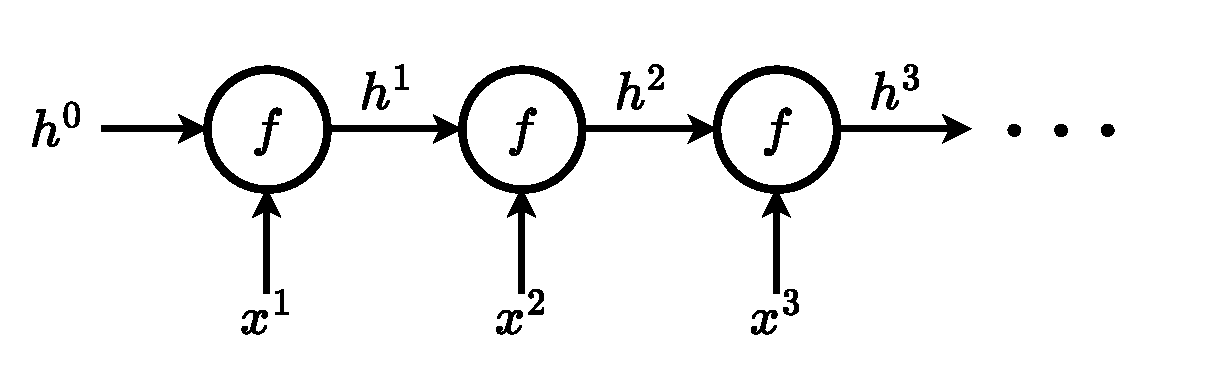
\includegraphics[width = 0.5\textwidth, height = 0.5\textheight, keepaspectratio]{images/chapter_7/rnn.pdf}
\end{figure}
    
\end{frame}


\begin{frame}[t]{Recurrent Neural Networks}

RNNs use a \textbf{hidden state}, passed as an additional input.
\vspace{10pt}

\begin{columns}
    \begin{column}{0.5\textwidth}
    \blist
        \item RNNs sequentially process inputs (i.e., first $x^1$ then $x^2$ $...$)
        \item The RNN also conditions on the \fat{hidden state} $h^t$
        \item $h^t$ can be thought of as a compact representation of the entire history of past inputs 
    \elist
    \end{column}
    \begin{column}{0.5\textwidth}
    \[
        \text{Function:\ } h^t = f(x^t, h^{t-1}; \theta)
    \]
    \begin{figure}
    \centering
    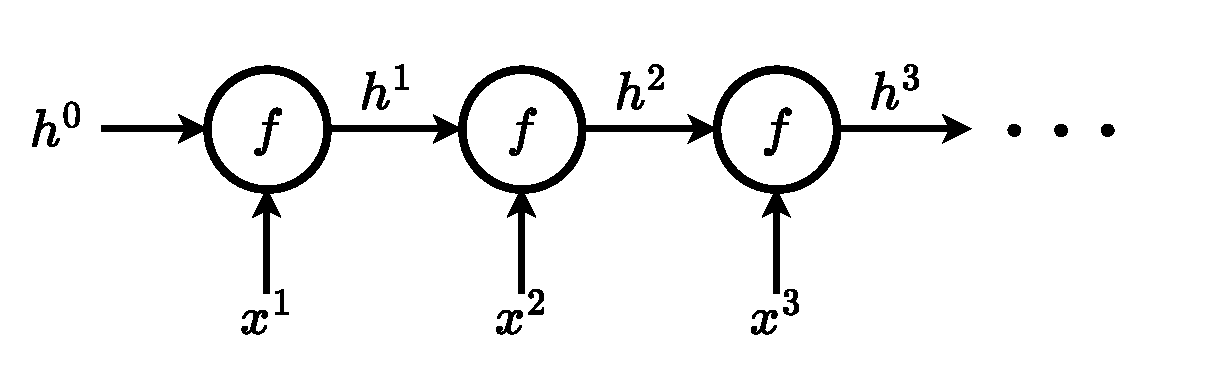
\includegraphics[width=0.9\textwidth]{images/chapter_7/rnn.pdf}
\end{figure}
    \end{column}
\end{columns}
\end{frame}


\begin{frame}{Summary}

\fat{We covered:}
    \blist
        \item Function approximation 
        \item Feed forward neural networks
        \item Loss functions, backpropagation and gradient descent
        \item CNNs and RNNs
    \elist

\fat{Next we'll cover:}

    \blist
        \item Deep \fat{reinforcement} learning 
    \elist
    
    
\end{frame}


\end{document}
